\chapter{BESIII实验上粲重子$\LtoXiXisK$的绝对分支比测量}
\label{chap:lambdac}

关于粲重子$\lambdacp$测量的背景情况我们在前言部分已经详细阐述过了,这里不再赘述。
重点提一下我们数据采集的能量点。
如图~\ref{fig:lambc_cs_belle}和图~\ref{fig:lambc_cs_bes3}所示,在各质心系能量下$\lambdacp\lambdacm$对过程产生的截面,在4.6$\gev$的质心系能量下Belle实验测量的结果为$\sigma(\ee\to\lambdacp\lambdacm)=0.38\pm0.13\,\rm{nb}$~\cite{Pakhlova:2008vn},BESIII初步的测量结果为$\sigma(\ee\to\lambdacp\lambdacm)=0.237\pm0.015\,\rm{nb}$~\cite{Ablikim:2017lct}。

\begin{figure*}[h]
\centering
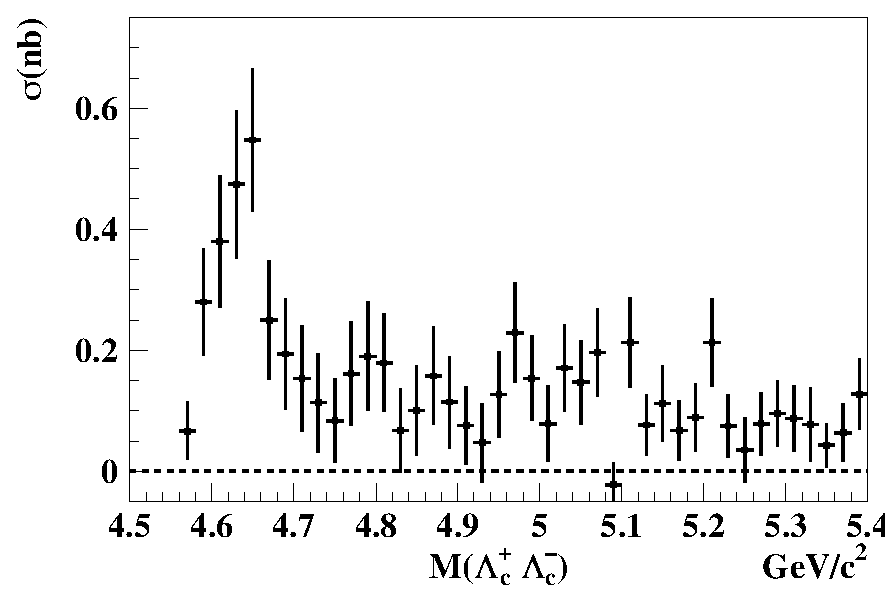
\includegraphics[width=0.85\textwidth]{chap2_LcLc_lineshape_belle}
\caption{ BELLE 实验测量的$\ee\to\lambdacp\lambdacm$ 的截面。}
\label{fig:lambc_cs_belle}
\end{figure*}

\begin{figure*}[h]
\centering
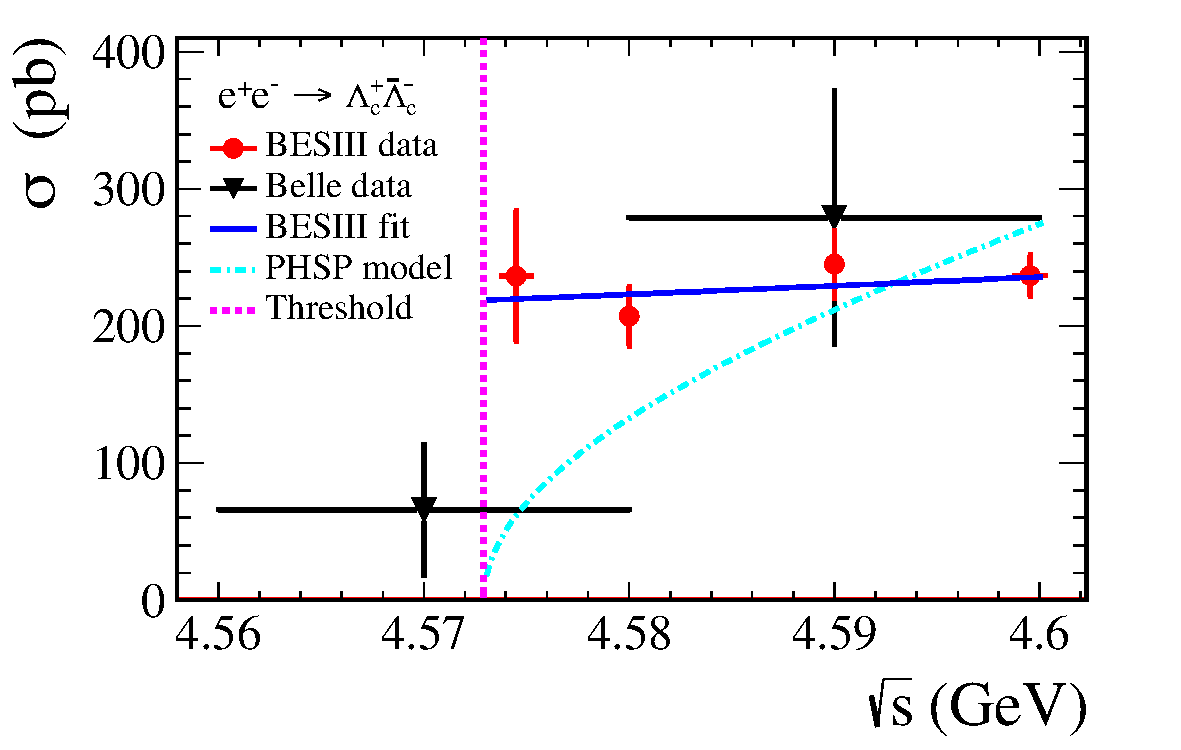
\includegraphics[width=0.85\textwidth]{chap2_LcLc_lineshape}
\caption{ BESIII 实验初步测量的$\ee\to\lambdacp\lambdacm$ 的截面。}
\label{fig:lambc_cs_bes3}
\end{figure*}
2014年BESIII在4.6$\gev$的质心系能量下进行取数,共积累了567$\rm{pb}^{-1}$的$\lambdacp\lambdacm$阈值数据。
我们知道$\lambdacp\lambdacm$的质量阈值为4573$\mev$,该能量点略高于$\lambdacp\lambdacm$对质量阈值26$\mev$左右。
注意到4.6$\gev$依然不是$\lambdacp\lambdacm$截面的峰值,但这却已经远远超过了北京正负电子对撞机II设计的最高能量4.2$\gev$。
不得不说BESIII实验能在$\lambdacp\lambdacm$的质量阈值以上采集数据这是BEPCII的巨大成功。
因为阈值上的数据本底简单,运动学约束的也比较好,同样情况下大家更愿意去相信阈值上数据给出的结果。
这批数据为我们研究测量$\lambdacp$的性质提供了一个非常好的平台。

